\chapter{Process Management and Scheduling}

Data is coming in at different, independent rate from sensors and is produced asynchronously from internal processing elements.
For certain processes, processing the incoming data as quickly as possible is key, however, this is challenging for several reasons:
1) a process may subscribe to multiple, independent streams with asychronized report schedules and 2) interpolated values
should be avoided to minimize prediction inaccuracies in interpolated values.  Therefore, a process actually wants all the freshest
data from all the streams they are subscribing to, while minimizing the average time that the data for each respective stream has 
been waiting in the buffer.

Sensor data is fundamentally challenging to deal with because much of it must be cleaned before it can be processed.  For example,
it is not uncommon to receive readings that is out of operational range, that is erroneous with respect to the previous observed trend,
or to stop receiving readings altogether.  This implies the need for processing jobs to provide a level of filtering over the raw streams.
Once the data is cleaned, it is typically consumed more sophisticated processes that aggregate the information or use it for control
of the space or equipment.  We provide the mechanisms for handling both classes of processing jobs with our process management layer.
In the next section we will discuss our process management layer and how users can both submit jobs to StreamFS for management or link
their own external processing elements so that they can be managed through StreamFS but run outside of StreamFS.

% \input{ProcessMngt}
\section{Internal Processes}
Internal processes are jobs submitted to StreamFS that are written in Javascript and managed within a StreamFS cluster.

StreamFS distinguishes between nodes that represent streaming data sources in the real-world
and those that do not.  Those that do not, however, can be tagged as aggregation points.  As part of the 
tagging processes, a user specifies the units of aggregation, with additional options for cleaning
and processing.  Our contributions are:  

\begin{itemize}
\item Use of the entity-relationship graph to provide OLAP \emph{roll-up}, \emph{drill-down},
		and \emph{slice and dice} operations.
\item Show how sliding-window operations can be used on real-time data in combination with the entity-relationship
		graph to maintain accurate aggregates as the underlying objects and inter-relationships change.
\end{itemize}


% \subsection{Mapping OLAP to ERG}
\subsection{OLAP-style Aggregation}

% \begin{itemize}
% \item Introduction to OLAP.
% \item Explanation of ERG in StreamFS.
% \end{itemize}
Online analytical processing (OLAP) is a processing layer that provides summurization of data
from a set of underlying data repository (date warehouses).  Traditionally, OLAP is used to process
business data.  Business data summurization allows an analyst ask targetted questions about aggregates 
and trends in their data.  The data is typically multidimensional in nature and operations can be performed with
respect to those dimensions and their inter-relationship.

\subsubsection{Measures, Dimenions, and Levels}
Measures are the value, dimensions are the units of measure as well as time, and levels/hierarchy are 
explicit in the naming structure.

\subsubsection{Operations: drill-down and roll-up}
Drill-down and roll-up are made explicit in the structure.  You can drill down to individual readings or roll them
up into an aggregation point at a particular level in the hierarchy.

\subsubsection{Operations: slice and dice}
Slice and dice operations 

\subsubsection{Operations: pivoting}
\subsection{Dynamic Aggregation}
\label{sec:dynagg}
Dynamic aggregation combines the underlying entity-relationship graph with in-network aggregation.  It treats
each node in the graph as a potential point of aggregation on a particular data type.  For example,
if we need to compute aggregates of \emph{KW} data and we declare the node for a particular room as
the point of aggregation, we accept data from all children of that node that, whose units are in \emph{KW},
and add the streams together over pre-defined window size or pre-defined timeouts.

The scheme is hiearchical, so a node only accepts data from its children and only sends data to its parent.
StreamFS checks for cycles when before node insertion and prevents double-counting errors by only allowing 
aggregation-points that are roots of a tree that is a sub-graph of the entity-relationship graph.  In our deployment,
each view is a managed as an independent hierarchy.  So the hierarchy of \emph{spaces} is separate from
the \emph{inventory} hierarchy or the \emph{taxonomy} hierarchy.  This allows us to ask questions with a particular
view in mind, without conflict, and is a natural fit for our aggregation scheme.

% \subsubsection{How it works}
Although there are different semantics applied to different node types at the application layer, StreamFS only knows
about two types of nodes: (1) default nodes and (2) stream nodes.  The main difference is that \emph{default} nodes
are not explicitly associated with data coming from a sensor and \emph{stream} nodes are.  Furthermore, default
nodes can have children, while stream nodes cannot.  In our application, meters are represented by default nodes
and each stream of data they produce is a stream node.

When an aggregation point is chosen and enabled, dynamic aggregation places a buffer at the node for the type
of data that should be aggregated.  If we want to aggregate \emph{KW} data, we specify the type and send an enable-aggregation
request to the node through an HTTP {\texttt POST} to the path for that node.  The flow of data starts at the leaves when
a stream node received data from a sensor through HTTP {\texttt POST}.  As data arrives it is immediately
forwarded upstream to the parent(s).  If a node that receives data from its children is an aggregation point it buffers
the data, otherwise it fowards it to its parent.

Ignoring the timeouts for now, lets imagine the parent is a point of aggregation and its buffer is full.  At this point
the parent separates data into bins for each source and cleans it for aggregation through interpolation.  The main
operation is to \emph{stretch} and \emph{fill} that data with linearly interpolated values.  The \emph{stretch}
operation orders all the timestamps in increasing order and for each bin (signal) interpolates the values using the
first (last) pair of data points.  If there is only a single data point, the stretch uses it as the missing value.
The \emph{fill} operation find the nearest timestamps that are less-than and greater-than the missing sampling time, 
uses their values to determine the equation of a line between them and interpolates the missing value using that equation.
Once this is done for each signal, the values are added together for each unqiue timestamp and the aggregated
signal is reported to the parent, where the operation occurs recursively to the root.
Figure~\ref{fig:aggtree} shows an illustration of its operation.  

%problem:  the buffer size has to increase exponentially up the tree, in order to not drop any values.
%solution: chuck the data into default-buffer sized pieces and parallelize the interpolation using the interpolated tasks technique


%FILL IN WITH REAL GRAPH
\begin{figure}[htb!]
\begin{center}
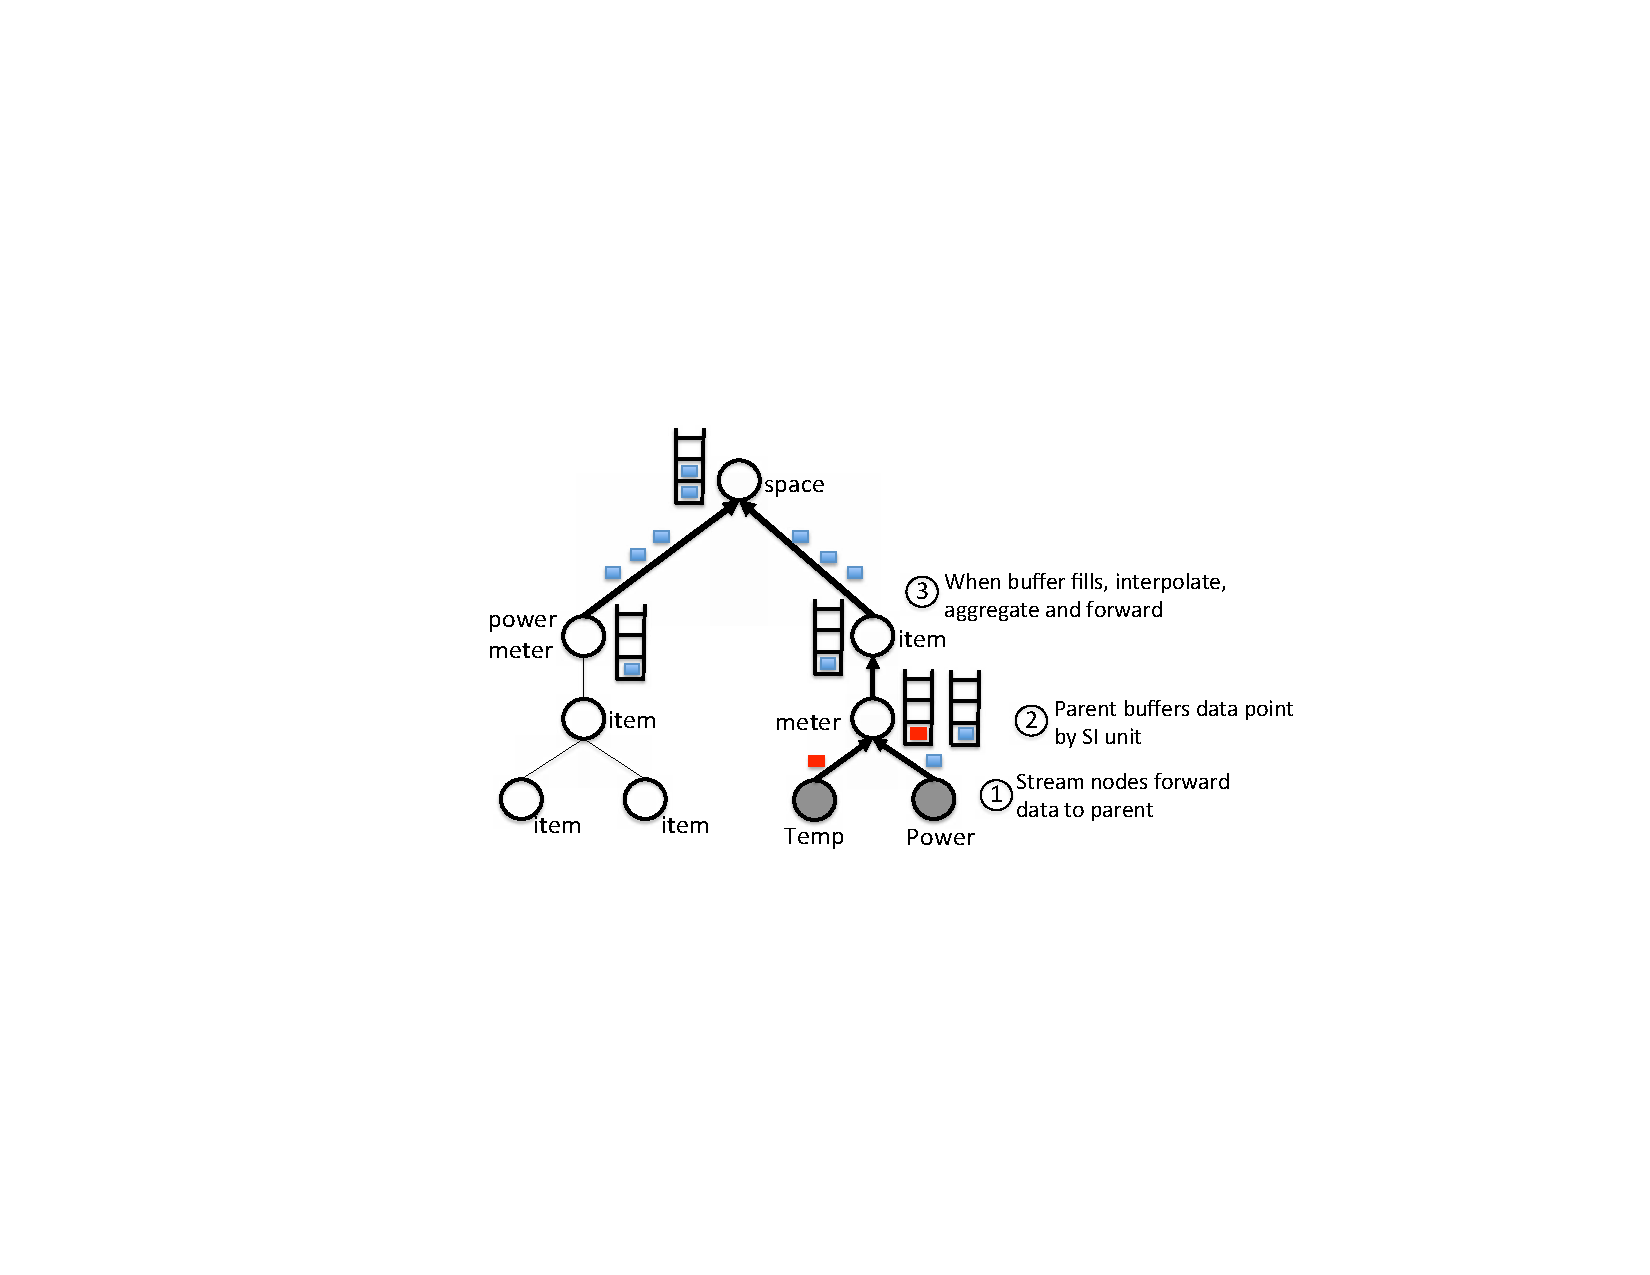
\includegraphics[scale=0.6]{figs/aggtree}
\caption{This shows an illustration of the aggregation tree used by \emph{dynamic aggregation}.  Data flows from 
the leaves to the root through user-specified aggregation points.  When the local buffer is full the streams
are separated by source, interpolated, and summed.  The aggregated signal is foward up the tree.}
\label{fig:aggtree}
\end{center}
\end{figure}

\subsubsection{Dealing with dynamics}
This approach deals with changes in the graph quite naturally.  All aggregation point deal only with local data, so
a node is only concerned about the children that give it data and the parent to send data to.  As objects in the environment
move from place to place and these changes are captured, the entity-relationship graph also changes to reflect the move.
This change in aggregation constituents is naturally accounted for in the aggregate.  If a child is removed,
it no longer forwards data to the old parent, therefore the aggregate will reflect that change.
Note, however, that changes in the entity-relationship graph are indistinguishable from energy-consuming items that have
been turned off.  For the purposes of aggregation, that is okay.

\subsubsection{Two scenarios}
We illustrate dynamic aggregation with a common usage scenario.  Imagine there are a number of people in a building,
each owning a number of plug-load applicances and a laptop.  Assume that when a person is in a room their laptop
is plugged in and when they leave the room they unplug their laptop and take it with them.  People come and go
throughout the day, changing the aggregate power consumption of the room and it happens.  In addition, some
of those people move to other rooms and plug their laptop in the new location.  As this happens, we will assume
all actions are being recorded in StreamFS.

%FILL IN WITH REAL GRAPH
\begin{figure}[htb!]
\begin{center}
\subfloat[Room 1 object and aggregate streams.]{%
            \label{fig:dynaggs1room1}
            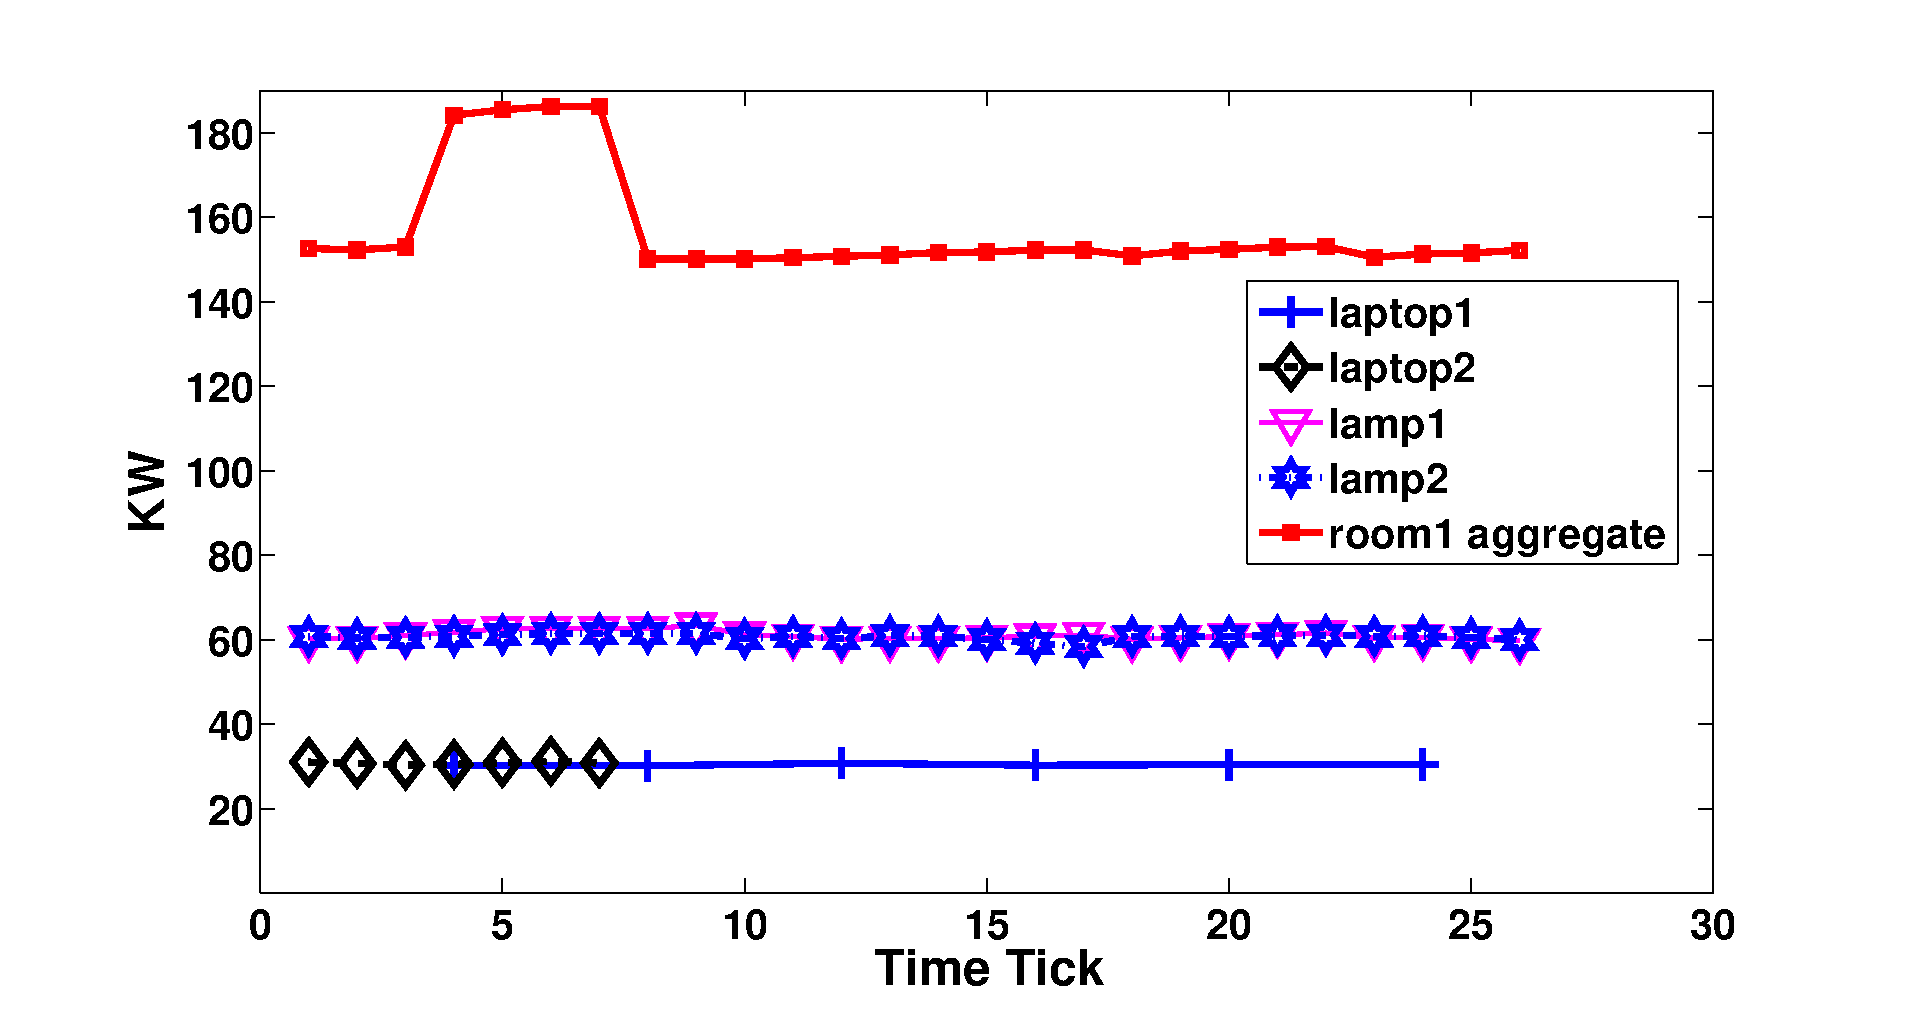
\includegraphics[scale=0.4]{figs/dynagg_scenario1_room1}
        }
\subfloat[Room 2 aggregate.]{%
            \label{fig:dynaggs1room2}
            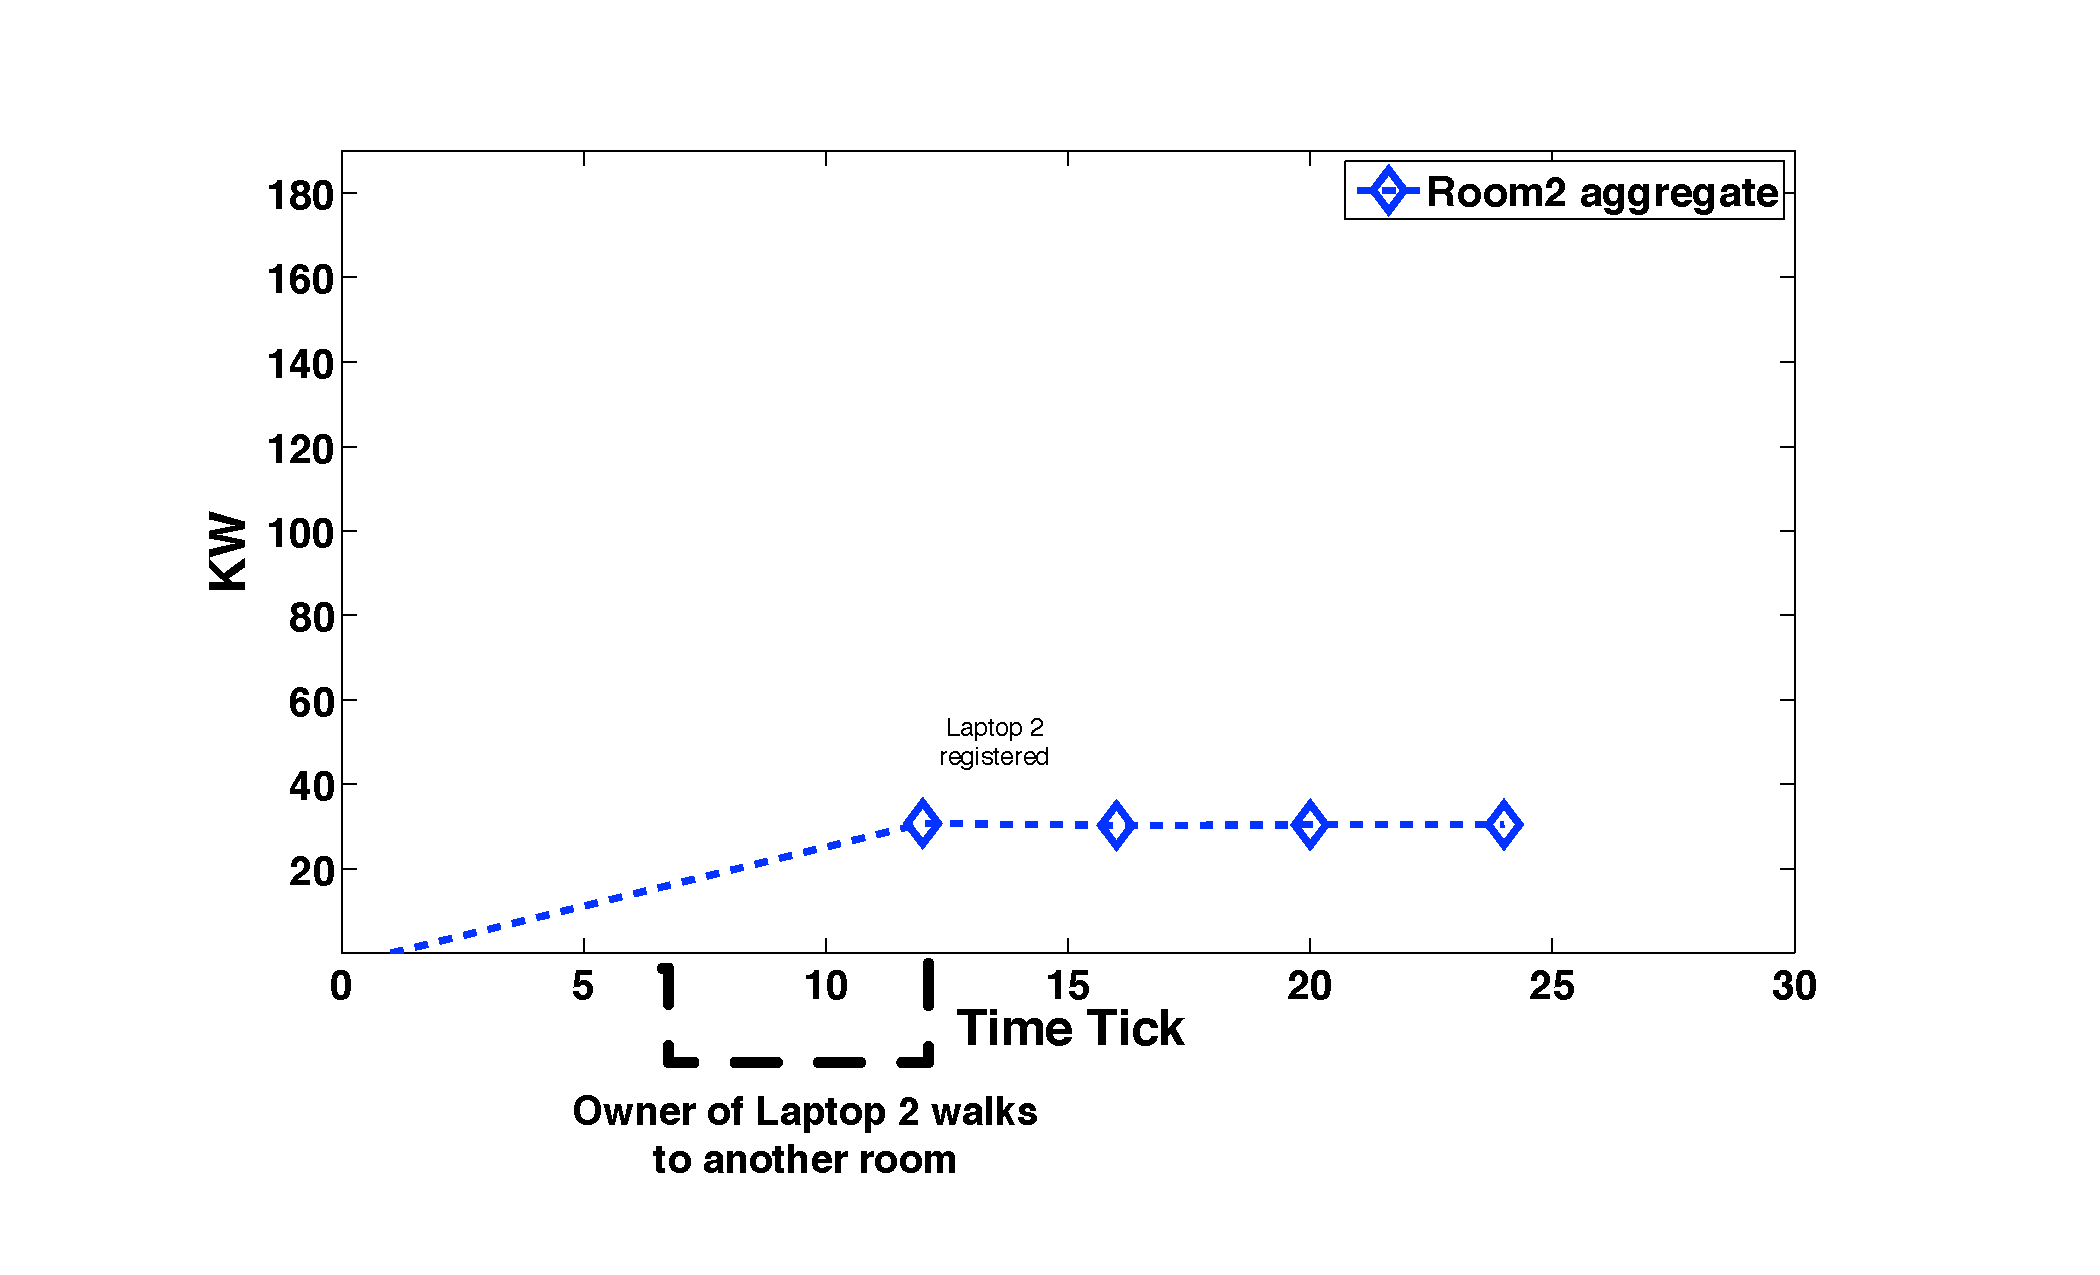
\includegraphics[scale=0.4]{figs/dynagg_scenario1_room2}
        }
\end{center}
\caption{
	The power consumes by a laptop in \emph{room 1} is shifted to \emph{room 2} a time t=7.  Notice the aggregagate drops in room 1
	while it rises in room 2.
     }%
\label{fig:multiroomagg}
\end{figure}

Figure~\ref{fig:multiroomagg} illustrate the aggregation results of that scenario.  Notice how...

% For demonstration lets have the user turn off on of their appliances when they leave as well.  This should cause that total
% room aggregate to drop, the person's personal aggregate to drop, but the other occupant's aggregate to remain
% the same.

% %FILL IN WITH REAL GRAPH
% \begin{figure}[htb!]
% \begin{center}
% 
\includegraphics[scale=0.39]{figs/blankbox}
% \caption{A room with items that belong to many users.  Person leaves with their item, aggregate falls.  Show aggregate.
% Person joins another room, aggregate in that room rises.  Show aggregate in the new room.  Compare before and after.}
% \label{fig:personaltotalagg}
% \end{center}
% \end{figure}

% Figure~\ref{fig:personaltotalagg} illustrate the results of the second sceanrio.  Note how...



\section{External Processes}

External processing jobs can be centrally managed in StreamFS as well.  In real deployments, it is often the case that
users do want to be limited by the particular libraries that are available to them in javascript or they have already made
a signficant investment in time writing and testing their own processing jobs.  We introduce an external client stub that 
re-directs data from standard in/out through a network connection to/from the StreamFS server.  The stub also interprets
process management commands to spawn and kill jobs and associate different subscriptions with different instances of a jobs 
running on the client side.

On startup, the client stub read a local configuration file that specifies the path to the job and metadata that describes
job.  These are used to register the job with StreamFS and set the metadata attributes.  The registration on the StreamFS 
server is exposed through an \emph{external process} file.  The user interact with an external job exactly the same way they
interact with an internal process job.  In order to spawn a job on the client, the user simply ``pipes'' a stream file 
to the external process file.  The creation of the pipe/subcription send a spawn message to the client and starts the associated
job on the client.  Once the process is started, data from the stream(s) is forwarded to the client, which writes it to the 
standard-in of the client job.  Starting a job also creates a stream file the StreamFS server.  Any data that's produced by the job
and written to standard-out is re-directed to the server and made available through the stream file.

This desgin is consistent with the semantics of pipe/subscription management and functionality.  Recall, internal processes
work the same way and this allow us to stay consistent with the file-centric principal whereby \emph{everything is managed
through the filesystem itself as a file}.



\section{Freshness Scheduling}
Process execution parameters are set by the user when a process element is created.  Generally, job scheduling is strictly driven
by these parameters.  However, in our deployments we found there were job pipe sinks that required a \emph{minimum freshness}
property for the set of data points in the buffer upon consumption.  In this section we discuss our scheduling algorithm in
relation to providing this property.% and present some experimental results.


\subsection{Maximizing Data Freshness}
\label{sec:freshness}

Data is coming in at different, independent rate from sensors and is produced asynchronously from internal processing elements.
For certain processes, the freshest
data from all the streams they are subscribing to is necessary; while minimizing the average time that the data for each respective 
stream has 
been waiting in the buffer.


\begin{algorithm}[h!]
 \SetAlgoLined
 Given a full buffer $b[n]$:\\
  \For{all elements in the $b$}{
  (1) Calculate the staleness of element $i$ and add to total staleness, $S_n$\;
  \For{all other elements in the buffer}{
    (1) Determine the next report time $D_i$ for this element\;
    (2) Determine the staleness of all the elements if we wait until $D_i$\;
    (3) If it is the smallest staleness figure calculate, replace minimum cost, $S_l$.
    }
  }
  \If{$S_l$ is less than $S_n$}{
  (1) Wait until later to consume\;
  \Else{
  (1) Consume now}
  }
 \caption{\texttt{min\_buffer} algorithm.}
 \label{alg:min_buffer}
\end{algorithm}


Some streams show lots of variability in its value distribution over time; driven by the underlying dynamics of the system being 
monitored.  For example, the power
consumption of an active server or laptop tends to have a varying power-draw profile over short time scales.  
For jobs doing aggregation of 
streaming data, it is often the case that the time when the last reading was received is very different across streams.  

\begin{figure}[t!] %htbp
\centering
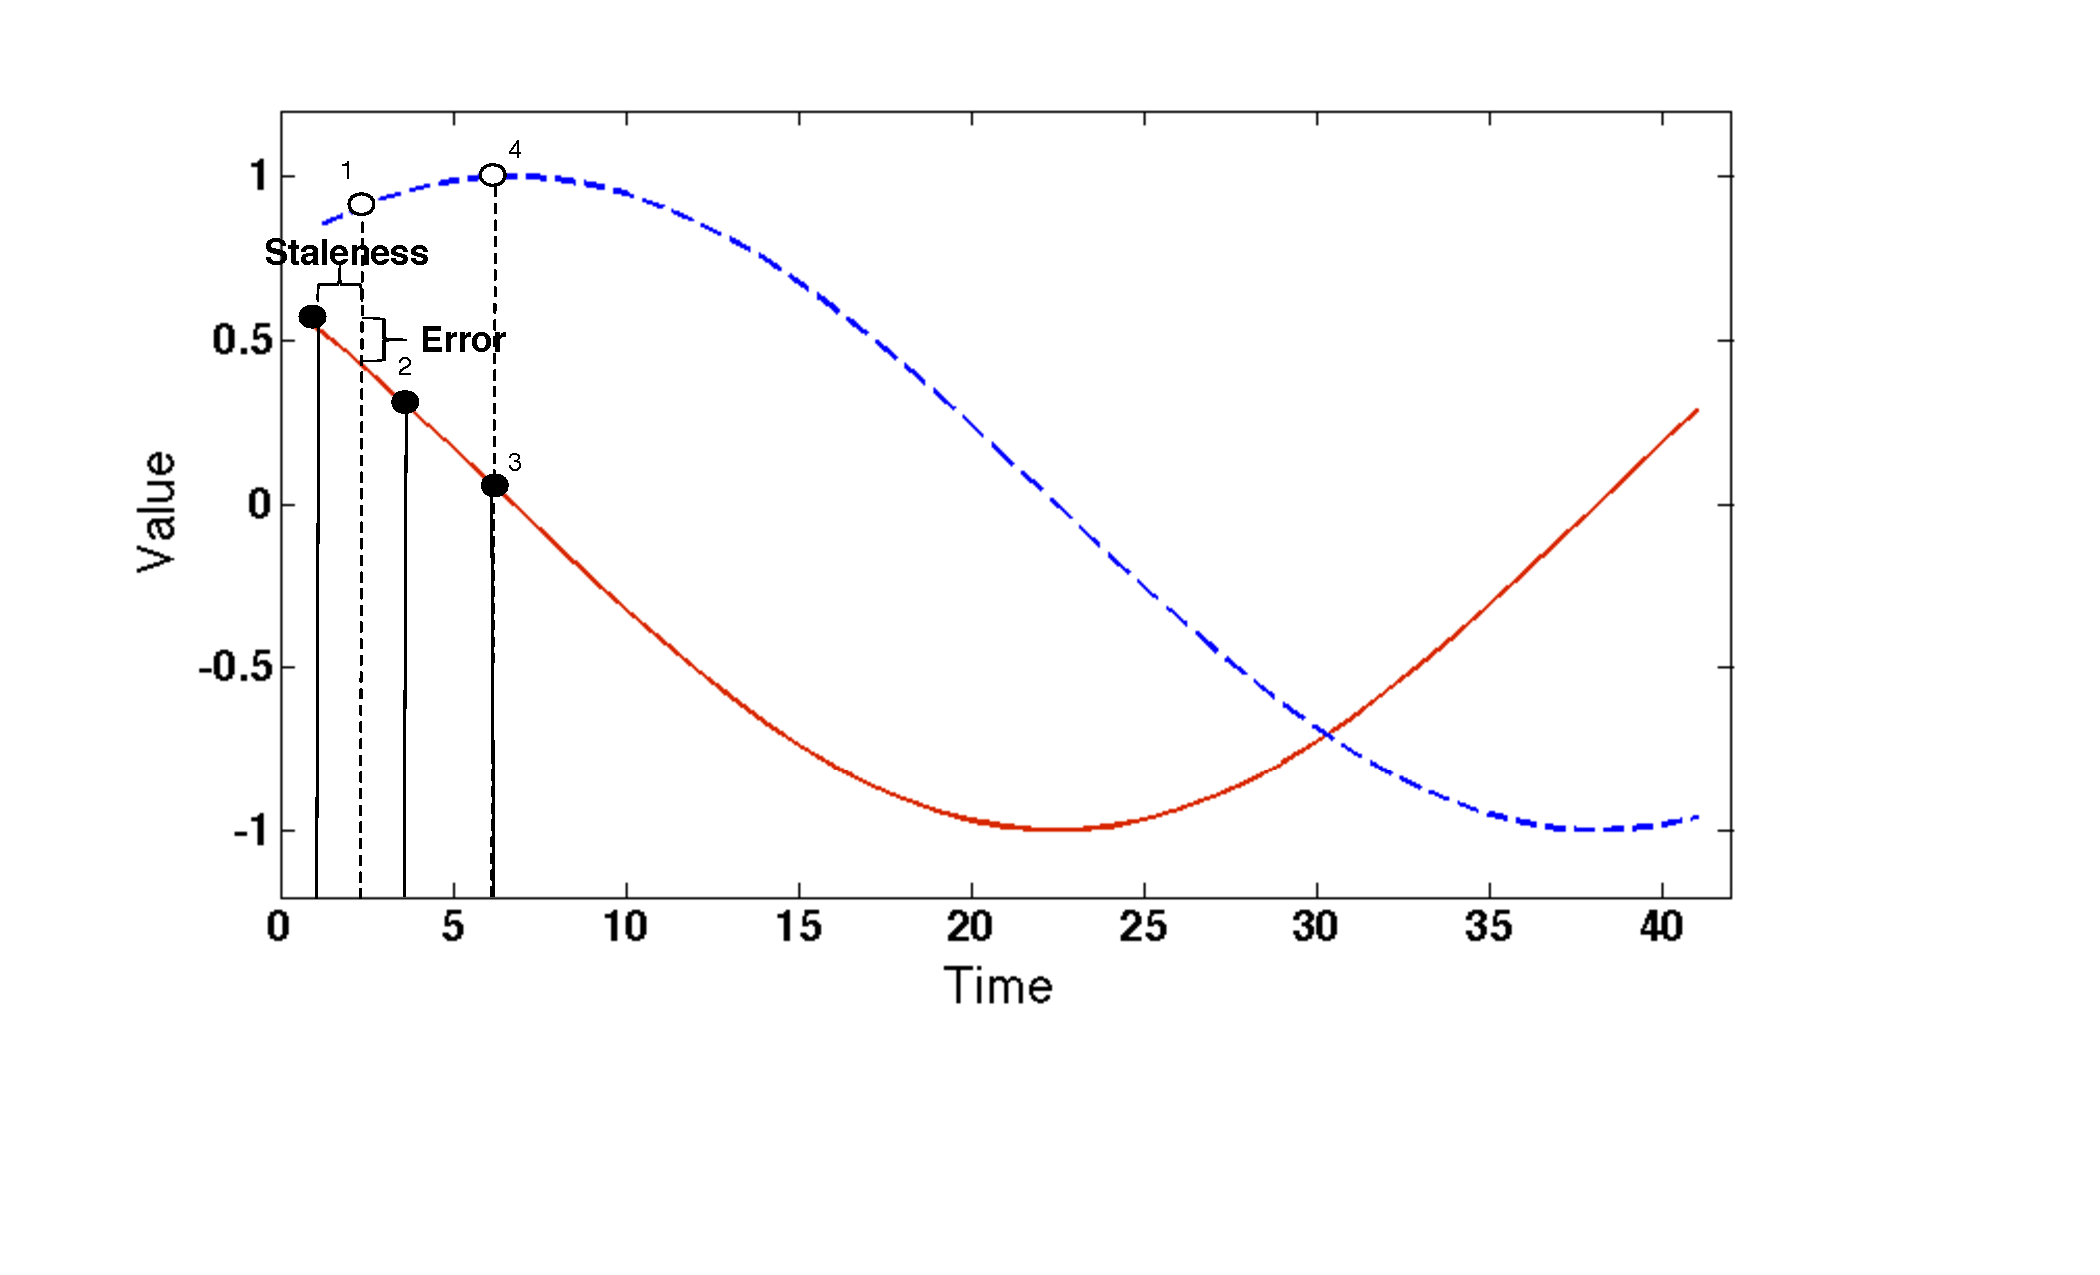
\includegraphics[width=0.75\columnwidth]{figs/sched_example.pdf}
\caption{This figure shows an example of two streams with different sampling frequencies.  Since we do not know the underlying fundamental frequency
of the phenomenon, our algorithm attempts to minimize error by minimizing staleness (or the average time a data point is in the receive buffer).}
\label{fig:sched_example}
\end{figure}

For example, consider two rapidly changing streams, as shown in Figure~\ref{fig:sched_example}.  
Each line represents the fundamental frequency of a different physical phenomenon.  The vertical lines represent reports times, as
observed at the StreamFS server; the time when the data points from those sensors are received.  
The circular dots show the value of the 
measurement that is in the buffer.  Assuming we have a subscriber that subscribes to only these two streams, the point labled with a 
`1' shows the first time that we can aggregate the two readings, `2' shows the second time, etc.
Note, the ideal aggregator \emph{minimizes} aggregation error in the sum, as specified in the figure.  Since a measurement was received 
at time t=2 and t=3, there will be some error associated with the sum -- the difference between the actual
value of the phenomenon at time t=3 and the value in the buffer (received at time t=2).  \emph{The longer we wait to compute the 
aggregate, the higher the error; until it resets when a new reading arrives}.

StreamFS does not know the underlying fundamental frequency of the phenomenon being measured, so it uses the staleness of the measurement to
approximate the error and a running report average for each stream to decide when it is best to compute the aggregate operation.  
Since the fundamental frequency is unknow, the driving assumption is that the more stale the reading, the higher the measurement error.  
Our measurement scheduler attempts to \emph{minimize aggregation error
by minimizing average buffer staleness} -- the time between the when the computation is taken and when the data point was received.  Note again
from the figure, that the best time to take a measurement is at t=6, since both data point come in at the same time and will have an average staleness
of 0.
% The ideal aggregation scenario is to
% combine the streams from the latest readings for both streams.  That way you minimizing the offset difference between during aggregation.
% If stream 1 produces a reading every three seconds and stream two produces a reading every two seconds, and you aggregate the readings every time you
% have at least one reading from both streams, every three seconds.  Sometimes the reading from the two-second stream will be one second old.
% If run the computation \emph{now}, the total staleness of the buffer is 1 second, if we wait on more second the total staleness is still one second, because
% at t=4 seconds, the three-second stream will be one second old.
For applications that wish to display the freshest aggregate (and approximate minimum error) we provide an algorithm
called \texttt{min\_buffer}.

The \texttt{min\_buffer} algorithm discards readings until two conditions are met:

\begin{enumerate}
\item There is at least one data point from each stream in the subscription buffer.
\item The staleness factor is minimized within the immediate time window.
\end{enumerate}

% This is of particular interest to controllers that need to make control decision based on the freshest data possible and can tolerate some variability
% in the completion time of the control task.  It is also useful in analytical jobs that want to process the latest data from multiple streams while also
% allowing some variability in the completion of the processing task.  
Note, there is a fundamental tradeoff
between the staleness factor and variability of consumption.  It is sometimes better to wait for the next incoming data point than it is to use what
is currently in the buffer, as waiting will decrease the overall staleness factor.  Other times, it is better to consume the buffered data immediately.
This causes a certain amount of variability in the delivery period to the control process.  However, for some applications, this is a reasonable tradeoff
to make.  Making use of the freshest data is desirable for minimizing errors, either in the control of a system or the calculation of some aggregate 
state.
Generally, the error grows with staleness, therefore the goal of this mechanism is to continuously minimize the error associated with staleness through
scheduling.


\begin{figure}[t!] %htbp
\centering
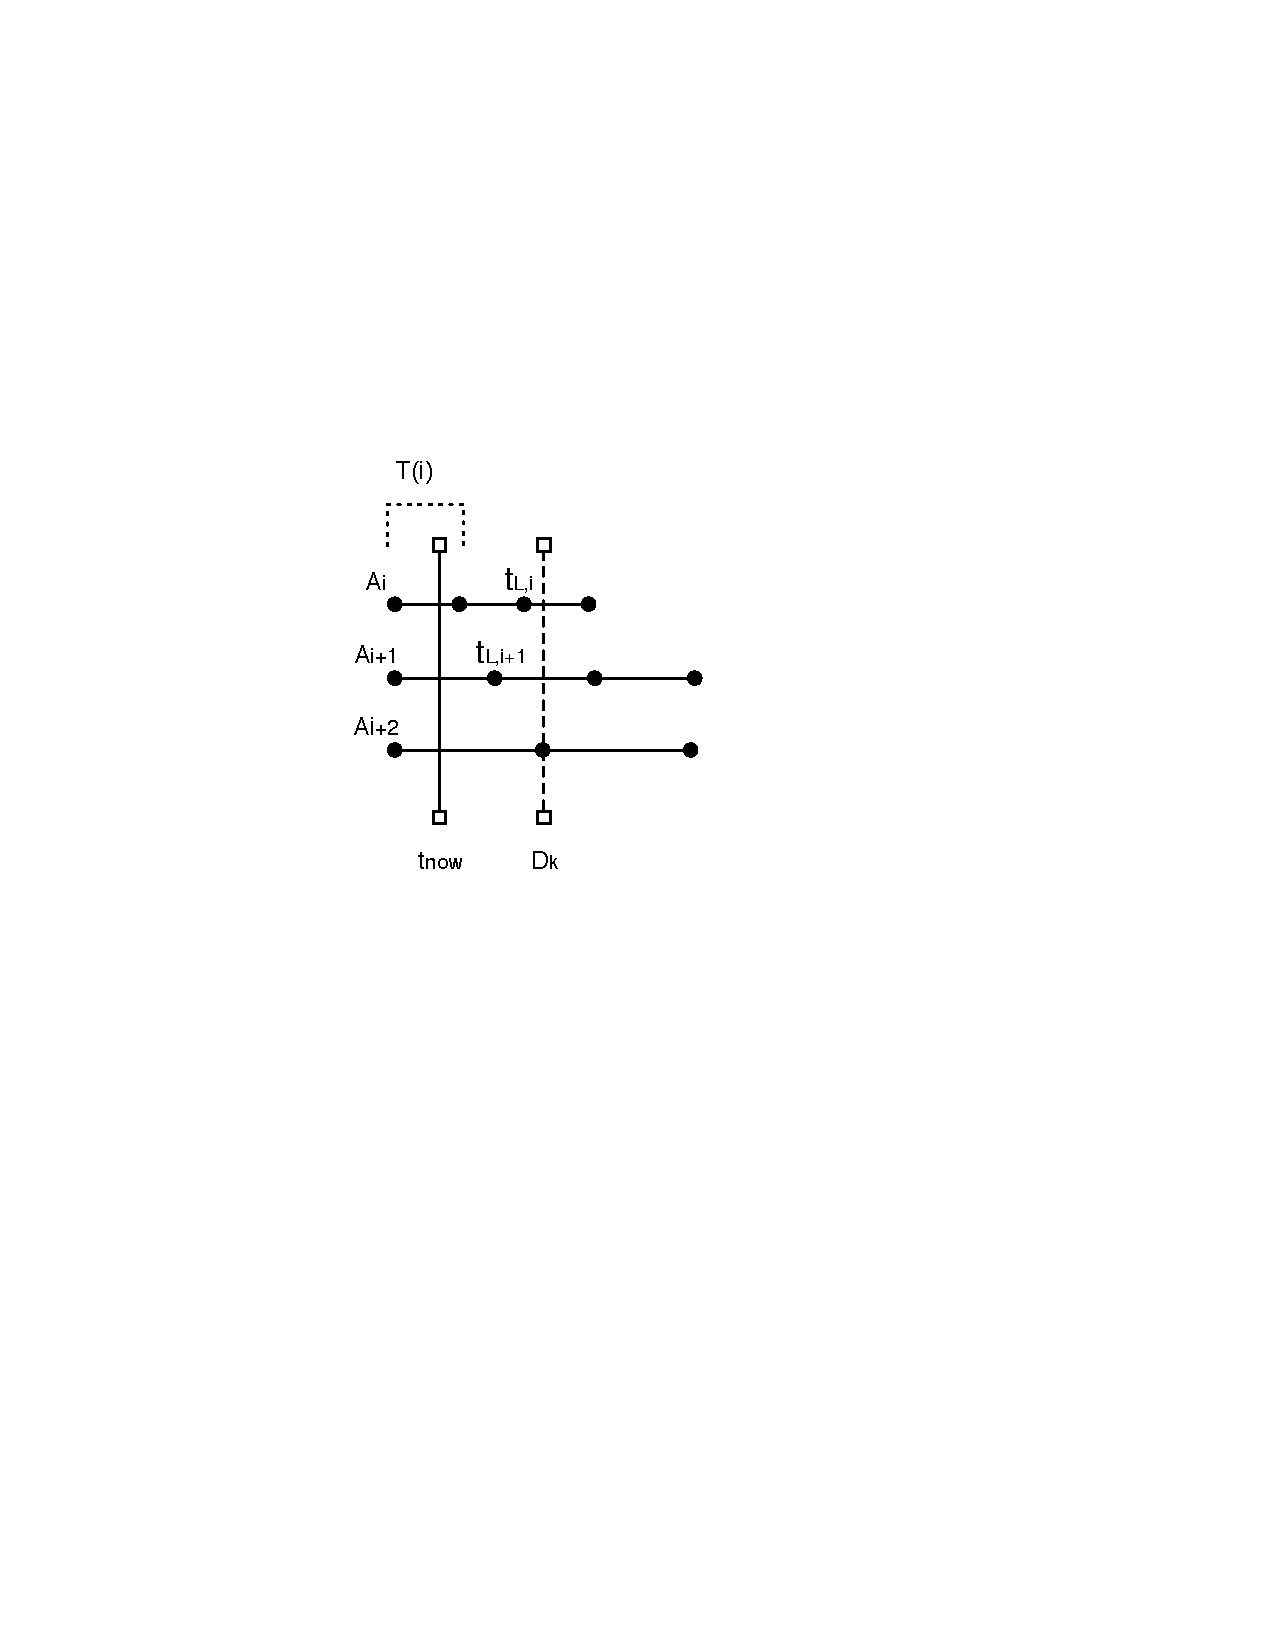
\includegraphics[width=0.75\columnwidth]{figs/min_buffer}
\caption{Multiple streams in a subscription and their associated parameters.}
\label{fig:min_buffer}
\end{figure}

Let $A_{i}$ be the arrival time of the last data point received from stream $i$ and $D_{i}$ be the arrival time for the next data point from stream $i$
and their relationship as described in Equation \ref{eqn:deadline}, where $T(i)$ is the average period between the arrivals from stream $i$.

\begin{equation}
D_{i} = A_{i} + T(i)
\label{eqn:deadline}
\end{equation}


Periodically, our algorithm runs and checks if there is a data point for each stream in the subscription.  If so, the \emph{min\_buffer} algorithm runs 
and effectively decides whether to execute the job on the current buffer immediately or whether to wait until later, when the \emph{staleness factor} of
the buffer will be at a minimum.  This decision is driven by Equation~\ref{eqn:later_better_condition}, whereby we find the next deadline, computed with
Equation~\ref{eqn:last_deadline}, for each stream in the set and determine the staleness factor will be for the entire buffer if we wait until that deadline arrives.

\begin{equation}
t_{L,i} = A_{i} + \Bigl\lfloor \frac{D_{k}-A_{i}}{T(i)} \Bigr\rfloor T(i)
\label{eqn:last_deadline}
\end{equation}

If there is no deadline $D_{k}$ for some stream $k$ such that Equation~\ref{eqn:later_better_condition} holds, then we execute now.  Otherwise we choose to wait
until $D_{k}$ for the stream whose next deadline minimizes the staleness factor of the buffer.


\begin{equation}
\sum_{i=1}^{k-1} D_{k} - t_{L,i} < \sum_{i=1}^{k} t_{now} - A_{i}
\label{eqn:later_better_condition}
\end{equation}

Algorithm~\ref{alg:min_buffer} shows the pseudocode for the \texttt{min\_buffer} algorithm.


\subsection{Results}

We test our hypothesis in this section by using EMD to remove low-frequency trends in the data
and run correlation calculation at overlapping IMF timescales.  We discover that EMD allows us
to find and compare high-frequency instrinsic behavior that is spatially correlated across
sensors.  We begin with a small set of three sensors (EHP, GHP, light) and expand our scope
to include all the sensors in the dataset.



\subsubsection{Initial analysis}
Lets consider the simple example of Section \ref{problem} where we would like to know if the EHP trace is correlated with the two other traces.
Recall that the correlation coefficients of the raw feeds was $0.7715$ and $0.6370$, corresponding to the light 
and GHP, respectively.
As stated in previous section this result is correct but not so meaningful, since most of the traces
display the same diurnal pattern.
Figure \ref{fig:emd} and Figure \ref{fig:emd2} show the EMD decomposition of the three traces.
For each trace, EMD has retrieved three IMFs that highlight the higher frequencies of the traces.

Figure~\ref{fig:emd} shows the normalized raw trace (top) and EMD output IMFs and residual as well as the 
correlation coefficients calculated on the IMFs for the EHP and
light traces.  The correlation coefficients are $0.43909$, $0.49344$ and $0.63469$ corresponding to the IMF1, 
IMF2, and IMF3, respectively.  Notice the high correlation between the high-frequency IMFs.
We know that the light and EHP serve the same room, and their high-frequency IMF correlation corroborates
our prior knowledge.
Figure~\ref{fig:emd2} shows a complementary result, for the EHP and GHP comparison.
The correlation coefficients for the EHP and GHP IMFs suggest that the two may be independent.  In fact, they
\emph{are} indepdent; they serve completely different rooms in the building!

EMD allows us to remove low-frequency trends that add noise to the original analysis.
By comparing IMFs, we see both intrisically correlated and \emph{uncorrelated} behavior.  In the next
section we expand our analysis and show the effectiveness of our methodology. 
% Although promising, these results must be validated across the rest of the
% dataset to confirm their significance.  


\subsubsection{Validation}
To validate the effectiveness of our approach, we analyze the same three-week time span for \emph{all} 674 
sensors deployed in the building.
For each trace $S$ we compute two scores: (1) the correlation coefficient between $S$ and the EHP trace
and (2) the average value of the IMF correlation coefficients.

\begin{figure}[tbh!]
\centering
 \subfloat[Raw traces correlation coefficients]{\label{fig:histo1}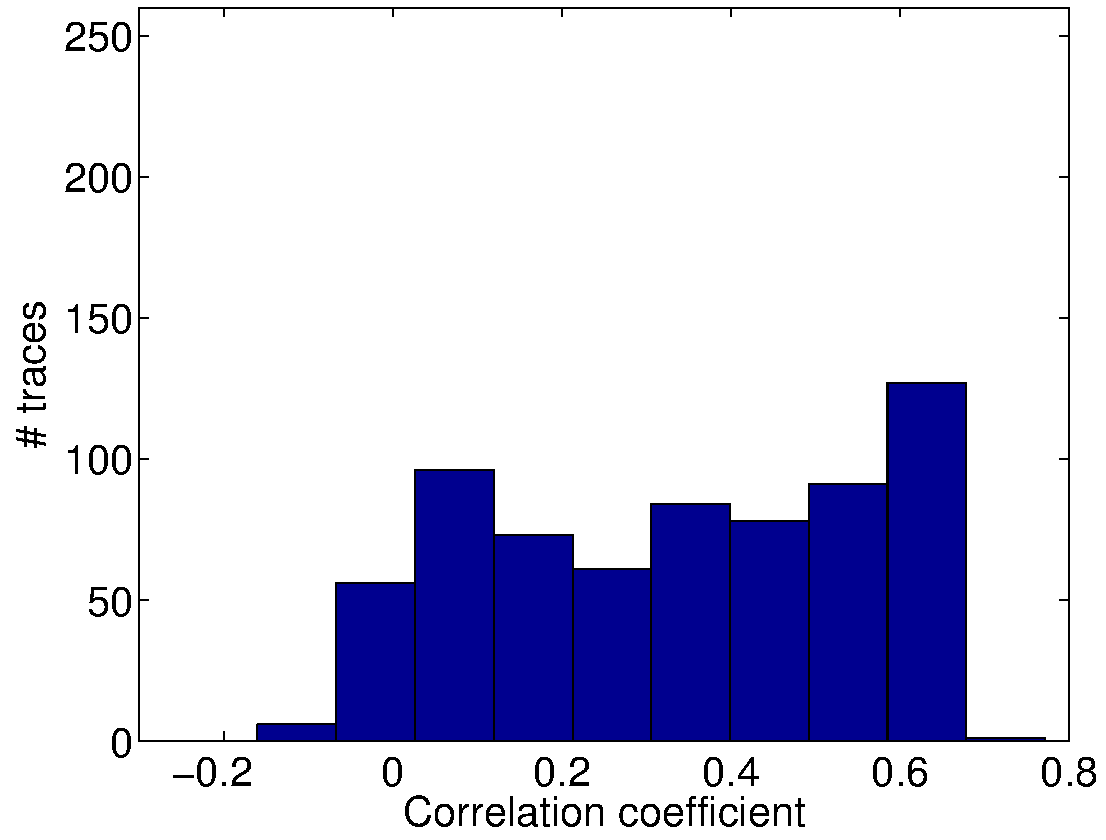
\includegraphics[width=.43\textwidth]{figs/allFloors_week1_week4_corr_abs-eps-converted-to}}
 \subfloat[Average IMFs correlation coefficients]{\label{fig:histo2}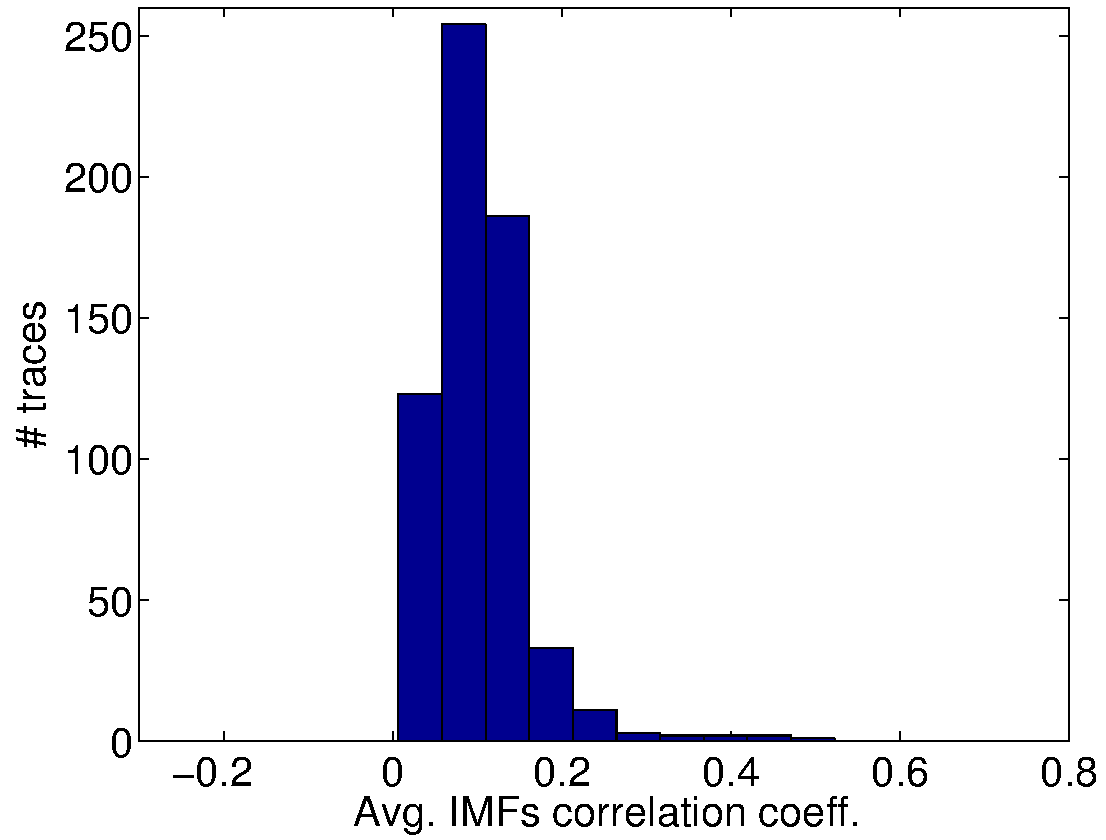
\includegraphics[width=.43\textwidth]{figs/allFloors_week1_week4_emd_abs-eps-converted-to}}
 \caption{Distribution of the correlation coefficients of the raw traces and correlation coefficients average of the corresponding IMFs using 3 weeks of data from 674 sensors.}
\label{fig:histo}
\end{figure}

\begin{figure}
\centering
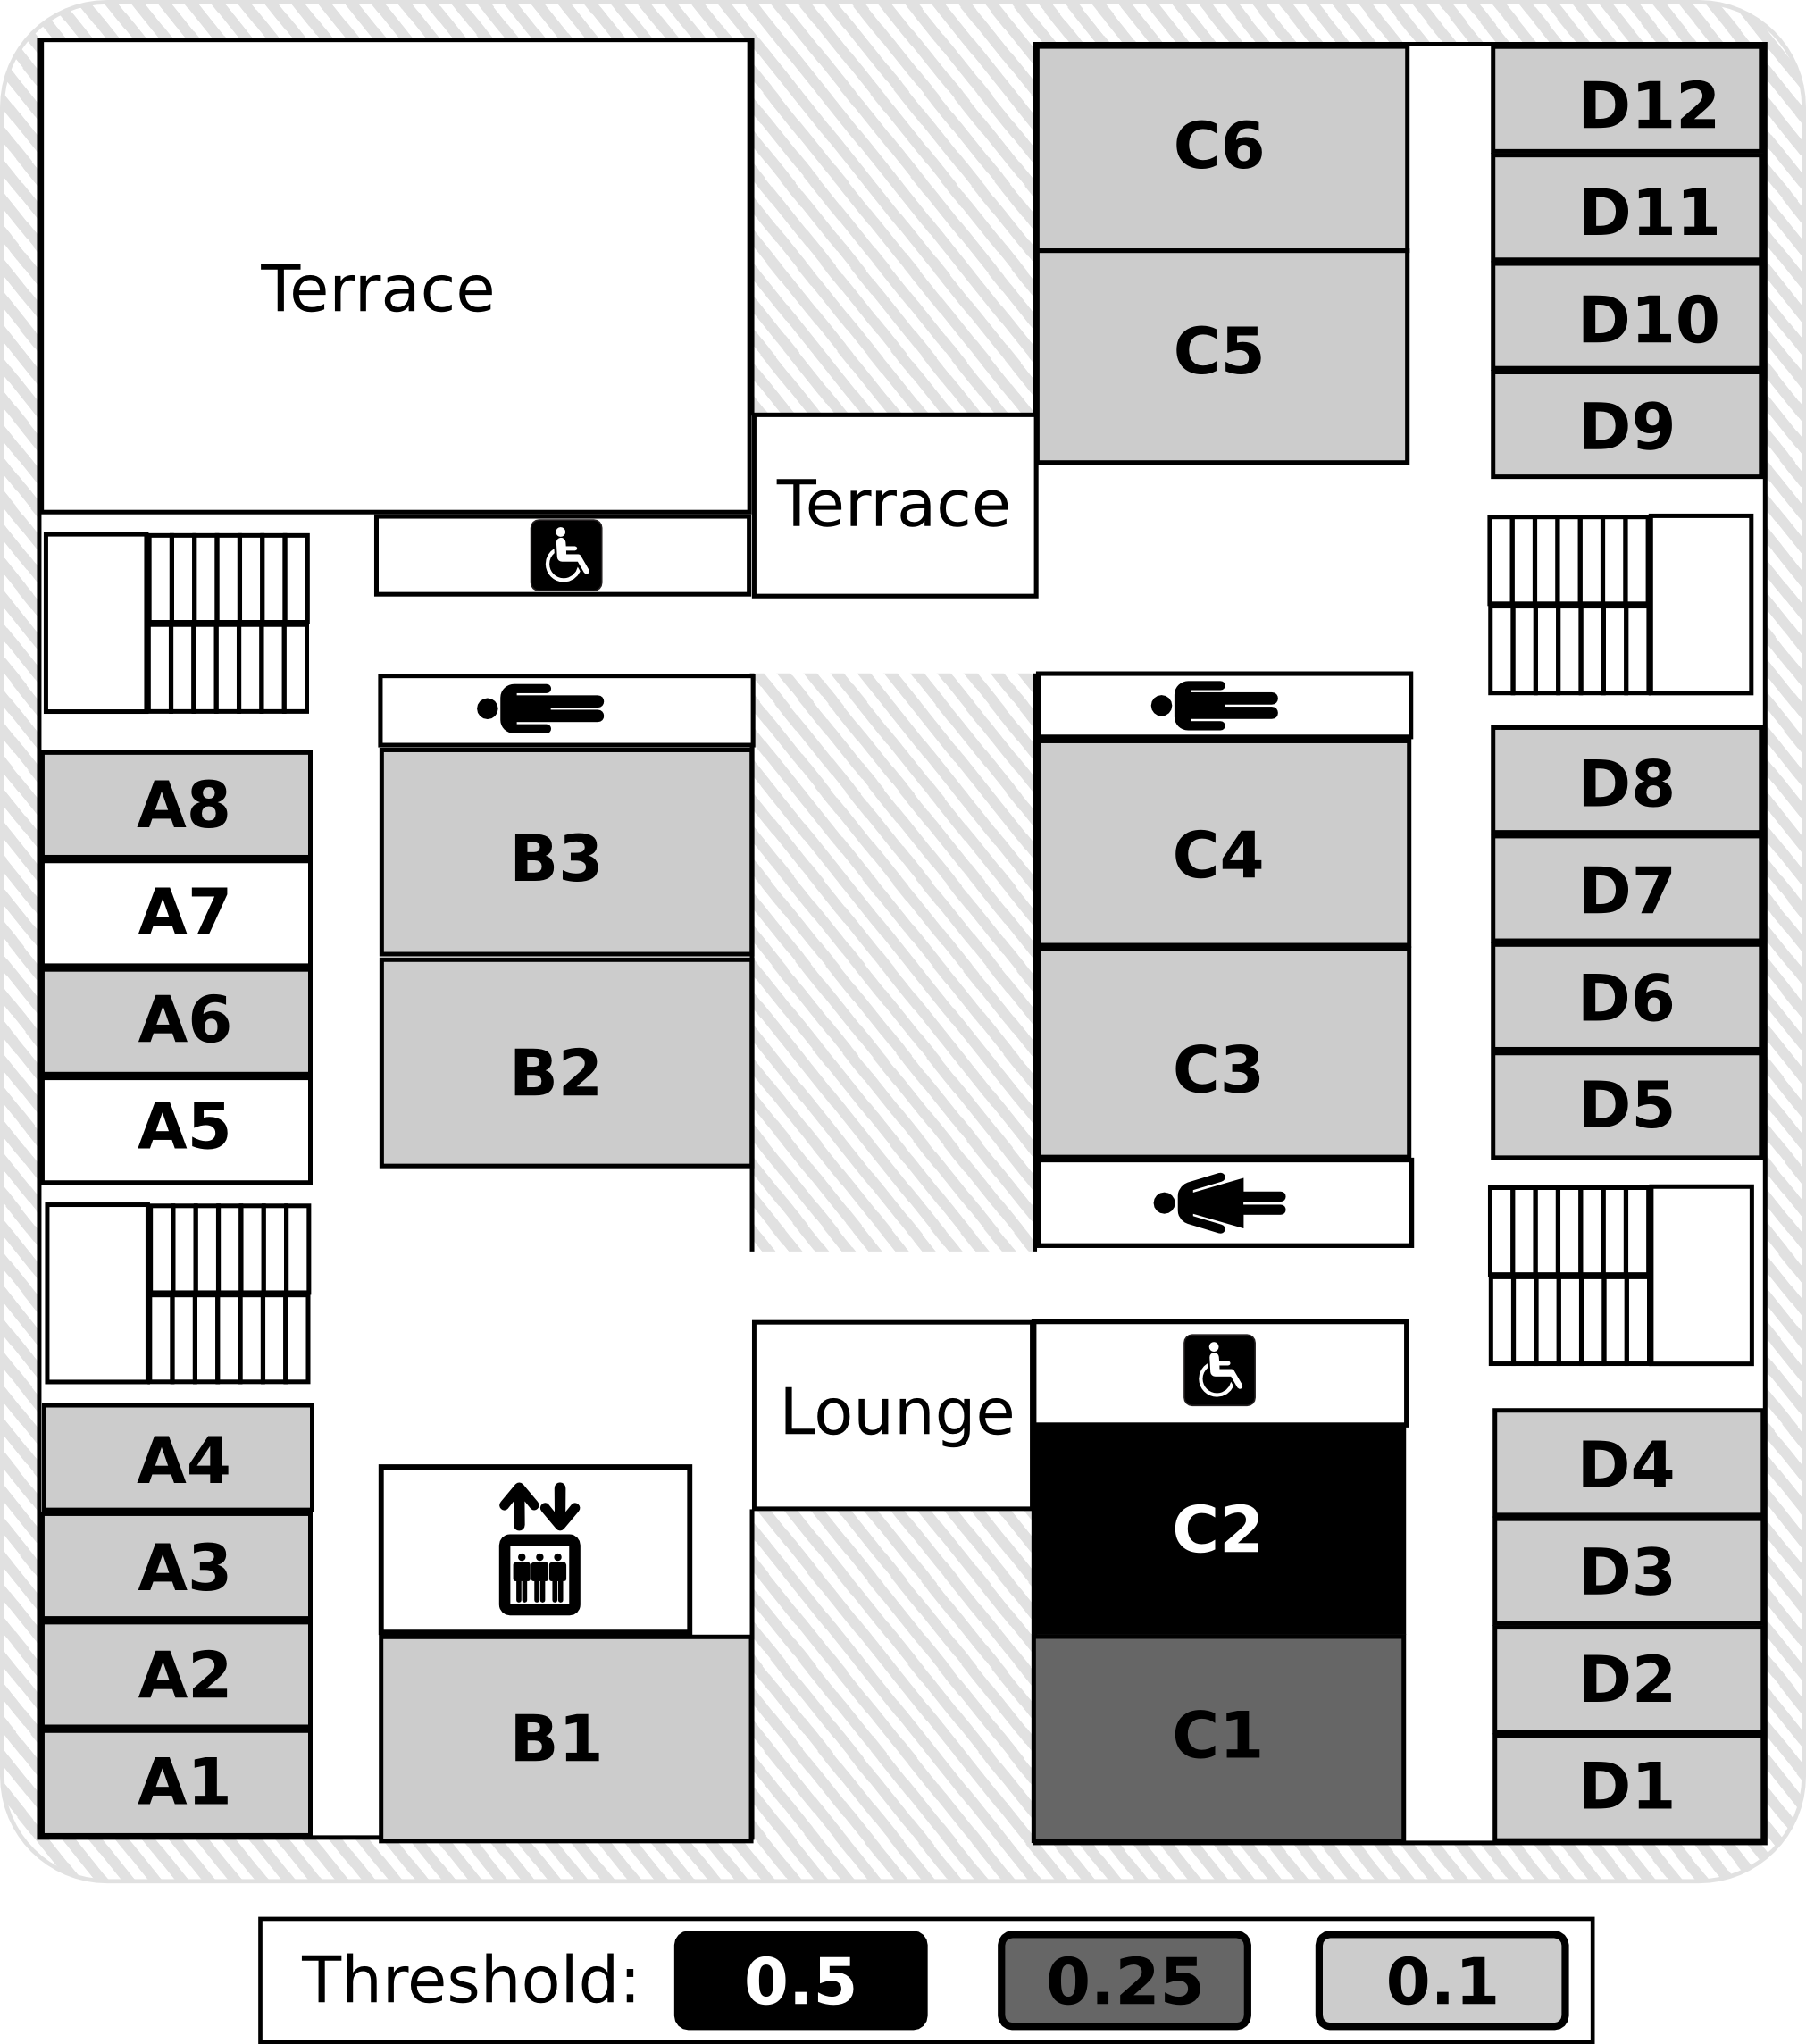
\includegraphics[width=.45\textwidth]{figs/floorMap.png}
\caption{Map of the floor where the analyzed EHP serves (room $C2$). The location of the sensors identified as related by the proposed approach are highlighted, showing a direct relationship between IMF correlation and spatial proximity.}
\label{fig:map}
\end{figure}

Figure \ref{fig:histo1} shows the distribution correlation coefficients.  Notice
that a large fraction of the dataset is correlated with the EHP trace.
\emph{Half} the traces have a correlation coefficient higher than $0.36$.  As expected, the underlying
trend is shared by a large number of device.
Although the highest score (i.e. $0.7715$) corresponds to the light in the same room that the EHP serves,
there are 118 pumps, serving all areas of the building, with a correlation higher than $0.6$.
Using only these results, it is not clear where the threshold should be set.  The distribution is close to 
uniform, making it difficult to 
know of how well your threshold discriminates against unrelated traces.
% Moreover, the distribution of the traces is almost uniform, thus, discriminating correlated traces is a laborious task.

Figure \ref{fig:histo2} shows the distribution of the average correlation value for the IMFs of
each trace and the EHP.  The number of traces correlated in the high frequency IMFs is significantly smaller
than the previous results. It's clear from the distribution that only a small set of devices are
\emph{intrinsically correlated} with the EHP.  In fact, \emph{only 10 traces out of 674} yielded a score higher than 
$0.25$. This allows us to easily rank traces by correlation.

Upon closer inspection of the 10 most correlated IMF traces, we find that there is a spatial relationship
between the EHP and the ten devices.  In fact, there is a direct relationship between score and distance from
the areas served by the EHP.  Figure~\ref{fig:map} shows a map of the floor that contains the rooms served by this
EHP.  The EHP directly serves room $C2$.  We introduce a correlation threshold to cluster correlated traces by score.
We highlight rooms by the threshold setting on the IMF correlation score.
When we set the threshold at $0.5$ we see that the sensors that have a correlation higher fall within room $C2$ --
the room served directly by the EHP.  As we relax the threshold, lowering it to $0.25$ and $0.1$ we see radial expansion from $C2$.  The trace with the highest score, $0.522$, is the trace corresponding to the lighting system \emph{in
the same room}.
The two highest scores for this floor (i.e. $0.316$ and $0.279$) are the light and EHP traces from next door, room $C1$.
Lower values correspond to sensors measuring activities in other rooms that have no specific relationship to the analyzed trace.  The results show a direct relationship between IMF correlation and spatial proximity and \emph{supports our initial
hypothesis}.


% Interestingly, the IMFs correlation coefficients reveal the spatial correlation of the sensors.
% Figure \ref{fig:map} is the map floor where the EHP trace is measured.
% Specifically, the EHP reports heating activity in the room $C2$.
% in the simple scenario the GHP is located in the room A5.



\section{Summary}

% StreamFS consists of over 20,000 lines of code and was implemented in mostly Java.  It was deployed across multiple
% buildings and several applications were built on top of it over a 2 years period.

In this chapter we gave an overview of the main components in StreamFS.  Each of the components addresses the concerns stated in 
section~\ref{sec:shortcomings}.  The filesystem name server expose a uniform namespace for access sensors and actuators in 
deployed throughout the building.  The timeseries database serve to store data streaming physical information and 
is optimized for the scan-style queries posed by applications.  These address points \ref{nw} and \ref{ts}.
We also include a pub-sub system which serves multiple purposes.  It provides real-time data forwarding for external
applications and forwards data internally to processing units that are specified or linked by the user.
This addresses points \ref{rt}.  Finally, we introduce processing elements, both internal and external to address
point \ref{proc}.  We also introduce an entity-relationship graph to deal with indirect relationships that are
expressed in the construction of names in the system.

In the next chapter we talk more about processing and discuss the details in the scheduler that help enable applications
that have certain delivery requirement.



